\documentclass[11pt]{article}
\usepackage{amsfonts}
\usepackage{amssymb}
\usepackage{geometry}
\usepackage{graphicx}
\usepackage{wrapfig}
\usepackage{tikz}
\usetikzlibrary{arrows.meta}
\usepackage{amsmath}
\usepackage{xcolor}
\usepackage[utf8]{inputenc}
\usepackage[T1]{fontenc}
\usepackage{caption}
\usepackage{fancyhdr}
\usepackage{fontawesome5}
\usepackage[inline]{enumitem}
\usepackage{array}
\usepackage[table]{xcolor}
\usepackage{colortbl}
\usepackage{mdframed}
\usepackage[most]{tcolorbox}
\tcbuselibrary{skins,breakable}
\usepackage{soul}
\definecolor{ncertblue}{RGB}{204, 232, 247}

\geometry{a4paper, margin=1in}

\fancypagestyle{firstpage}{
    \fancyhf{}
    \fancyhead[L]{
\includegraphics[width=0.2\textwidth]{../../iiitb_logo.png}
    \fancyhead[R]{%
        \begin{tabular}{r}
            \textbf{Name:} Pirjade Sabahat Rehan\\
            \textbf{ID:} COMETFWC056\\
            \textbf{Date:} January 26, 2026
        \end{tabular}
    }
    \renewcommand{\headrulewidth}{\pagestyle{plain}
\begin{document}
\thispagestyle{firstpage}
\vspace*{0.5cm}
\begin{center}
    \Large\textcolor{cyan}{\textbf{\large RELATIONS AND FUNCTIONS}}
\end{center}
\begin{center}
\begin{tcolorbox}[
  enhanced,
  width=0.25\textwidth,   
  colback=cyan!20,
  colframe=cyan!80!black,
  boxrule=1.2pt,
  arc=0mm,                
  left=10pt,
  right=10pt,
  top=8pt,
  bottom=8pt
]
\centering
\textbf{\textcolor{cyan!80!black}{EXERCISE 2.1}}
\end{tcolorbox}
\end{center}
\noindent 1. If $\left(\frac{x}{3}+1, y-\frac{2}{3}\right)=\left(\frac{5}{3}, \frac{1}{3}\right)$, find the values of $x$ and $y$.

\noindent 2. If the set $A$ has 3 elements and the set $B=\{3,4,5\}$, then find the number of elements in $(A\times B)$.
\noindent 3. If $G=\{7,8\}$ and $H=\{5,4,2\}$, find $G\times H$ and $H\times G$.

\noindent 4. State whether each of the following statements are true or false. If the statement is false, rewrite the given statement correctly.
\begin{itemize}
    \item[(i)] If $P=\{m,n\}$ and $Q=\{n,m\}$, then $P\times Q=\{(m,n),(n,m)\}$.
    \item[(ii)] If $A$ and $B$ are non-empty sets, then $A\times B$ is a non-empty set of ordered pairs $(x, y)$ such that $x\in A$ and $y\in B$.
    \item[(iii)] If $A=\{1,2\}$, $B=\{3,4\}$, then $A\times(B\cap\phi)=\phi$.
\end{itemize}

\noindent 5. If $A=\{-1,1\}$, find $A\times A\times A$.

\noindent 6. If $A\times B=\{(a,x),(a,y),(b,x),(b,y)\}$, find $A$ and $B$.

\noindent 7. Let $A=\{1,2\}$, $B=\{1,2,3,4\}$, $C=\{5,6\}$ and $D=\{5,6,7,8\}$. Verify that:
\begin{itemize}
    \item[(i)] $A\times(B\cap C)=(A\times B)\cap(A\times C)$
    \item[(ii)] $A\times C$ is a subset of $B\times D$.
\end{itemize}

\noindent 8. Let $A=\{1,2\}$ and $B=\{3,4\}$. Write $A\times B$. How many subsets will $A\times B$ have? List them.

\noindent 9. Let $A$ and $B$ be two sets such that $n(A)=3$ and $n(B)=2$. If $(x, 1), (y, 2), (z, 1)$ are in $A\times B$, find $A$ and $B$.

\noindent 10. The Cartesian product $A \times A$ has 9 elements among which are found $(-1, 0)$ and $(0,1)$. Find the set $A$ and the remaining elements of $A \times A$.
\textcolor{cyan}{\section*{2.3 Relations}}

\begin{wrapfigure}[14]{r}{0.40\textwidth}
\centering
\vspace{-25pt} 
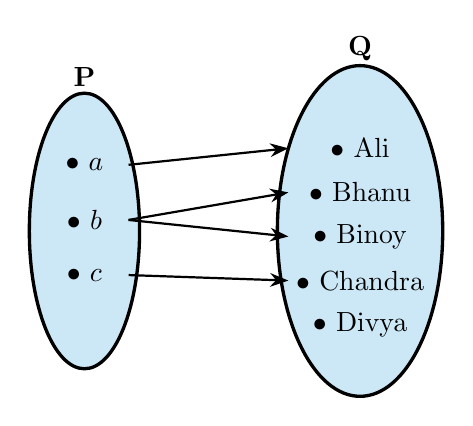
\begin{tikzpicture}[>=Stealth, scale=0.7]
% LEFT SET P
\draw[very thick, fill=ncertblue] (-2.5,0) ellipse (1.0 and 2.5);
\node at (-2.5,2.8) {\textbf{P}};
\node (a) at (-2.5,1.2) {$\bullet\ a$};
\node (b) at (-2.5,0.2) {$\bullet\ b$};
\node (c) at (-2.5,-0.8) {$\bullet\ c$};

\draw[very thick, fill=ncertblue] (2.5,0) ellipse (1.5 and 3.0);
\node at (2.5,3.3) {\textbf{Q}};
\node (ali) at (2.5,1.5) {$\bullet$ Ali};
\node (bha) at (2.5,0.7) {$\bullet$ Bhanu};
\node (bin) at (2.5,-0.1) {$\bullet$ Binoy};
\node (cha) at (2.5,-0.9) {$\bullet$ Chandra};
\node (div) at (2.5,-1.7) {$\bullet$ Divya};

\draw[->, thick] (-1.7,1.2) -- (1.2,1.5);
\draw[->, thick] (-1.7,0.2) -- (1.2,0.7);
\draw[->, thick] (-1.7,0.2) -- (1.2,-0.1);
\draw[->, thick] (-1.7,-0.8) -- (1.2,-0.9);
\end{tikzpicture}
\caption*{\textbf{Fig 2.4}}
\end{wrapfigure}

Consider the two sets $P = \{a, b, c\}$ and $Q = \{\text{Ali, Bhanu, Binoy, Chandra, Divya}\}$. The Cartesian product of $P$ and $Q$ has 15 ordered pairs: $P \times Q = \{(a, \text{Ali}), (a, \text{Bhanu}), \dots, (c, \text{Divya})\}$. 

\vspace{0.5em}
We can now obtain a subset of $P \times Q$ by introducing a relation $R$ as:
$R = \{ (x,y) : x \text{ is the first letter of the name } y, x \in P, y \in Q \}$. 

\vspace{0.5em}

Then $R = \{(a, \text{Ali}), (b, \text{Bhanu}), (b, \text{Binoy}), (c, \text{Chandra})\}$.
An arrow diagram of this relation $R$ is shown in Fig.~2.4.

\vspace{0.8em}

\vspace{0.8em}

\noindent
\colorbox{ncertblue}{\textcolor{cyan}{\textbf{Definition 2}}}\hspace{0.5em}
A relation $R$ from a non-empty set $A$ to a non-empty set $B$ is a subset of
the cartesian product $A \times B$. The subset is derived by describing a
relationship between the first element and the second element of the ordered
pairs in $A \times B$. The second element is called the \textit{image} of the
first element.

\vspace{0.6em}
\noindent
\colorbox{ncertblue}{\textcolor{cyan}{\textbf{Definition 3}}}\hspace{0.5em}
The set of all first elements of the ordered pairs in a relation $R$ from a set
$A$ to a set $B$ is called the \textit{domain} of the relation $R$.

\vspace{0.6em}
\noindent
\colorbox{ncertblue}{\textcolor{cyan}{\textbf{Definition 4}}}\hspace{0.5em}
The set of all second elements in a relation $R$ from a set $A$ to a set $B$ is
called the \textit{range} of the relation $R$. The whole set $B$ is called the
\textit{codomain} of the relation $R$. Note that range $\subset$ codomain.

\vspace{0.6em}
\noindent
\colorbox{ncertblue}{\textcolor{cyan}{\textbf{\textit{Remarks}}}}

\begin{enumerate}
\item A relation may be represented algebraically either by the
\textit{Roster method} or by the \textit{Set-builder method}.
\item An arrow diagram is a visual representation of a relation.
\end{enumerate}

\noindent\textcolor{cyan}{\textbf{Example 7}}

\textbf Let $A=\{1,2,3,4,5,6\}$. Define a relation $R$ from $A$ to $A$ by 
$R=\{(x,y):y=x+1\}$
\begin{enumerate}
    \item[(i)] Depict this relation using an arrow diagram.
    \item[(ii)] Write down the domain, codomain and range of $R$.
\end{enumerate}
\noindent\textcolor{cyan}{\textbf{Solution}}
\noindent
\begin{minipage}[t]{0.58\textwidth}
\begin{enumerate}[label=(\roman*), leftmargin=1.5em, nosep]
\item By the definition of the relation,
\[
R=\{(1,2),(2,3),(3,4),(4,5),(5,6)\}.
\]
The corresponding arrow diagram is shown in Fig.~2.5.

\item We can see that the domain $=\{1,2,3,4,5\}$.  
Similarly, the range $=\{2,3,4,5,6\}$ and the codomain
$=\{1,2,3,4,5,6\}$.
\end{enumerate}
\end{minipage}
\hfill
\begin{minipage}[t]{0.38\textwidth}
\vspace{0pt} 
\centering

\includegraphics[width=\linewidth]{task/2.5.jpg}
\end{minipage}
\vspace{0.6cm}
\textcolor{cyan}{\textbf{Example 8}}
 The Fig 2.6 shows a relation between the sets $P$ and $Q$. Write this relation 
\begin{enumerate}
    \item[(i)] in set-builder form, 
    \item[(ii)] in roster form. 
\end{enumerate}
What is its domain and range?
\vspace{0.35cm}
\textcolor{cyan}{\textbf{Solution}}  
It is obvious that the relation $R$ is “$x$ is the square of $y$”.

\medskip

\noindent
\begin{minipage}[t]{0.58\textwidth}

\begin{enumerate}
\item[(i)] \textbf{In set-builder form,}
\[
R = \{(x,y) : x \text{ is the square of } y,\ x \in P,\ y \in Q\}
\]

\item[(ii)] \textbf{In roster form,}
\[
R = \{(9,3),(9,-3),(4,2),(4,-2),(25,5),(25,-5)\}
\]
\end{enumerate}

The domain of this relation is $\{4,9,25\}$.\\
The range of this relation is $\{-2,2,-3,3,-5,5\}$.\\
Note that the element $1$ is not related to any element in set $P$.
The set $Q$ is the codomain of this relation.

\end{minipage}
\hfill
\begin{minipage}[t]{0.38\textwidth}
\vspace{0pt} 
\centering

\includegraphics[width=\linewidth]{task/2.6.jpg}

\end{minipage}
\begin{tcolorbox}[
  enhanced,
  breakable,
  width=\textwidth,       
  colback=cyan!15,
  colframe=cyan!70!black,
  boxrule=1.2pt,           
  arc=2mm,
  left=16pt,              
  right=16pt,
  top=12pt,
  bottom=12pt,
  before skip=10pt,
  after skip=12pt
]

\textbf{\textcolor{cyan!70!black}{\faHandPointRight\ Note}}\quad
The total number of relations that can be defined from a set $A$ to a set $B$
is the number of possible subsets of $A \times B$. If $n(A)=p$ and $n(B)=q$, then

$n(A \times B)=pq$
and the total number of relations is $2^{pq}$.

\end{tcolorbox}


\vspace{0.75cm}


\noindent\textcolor{cyan}{\textbf{Example 9}}
Let $A = \{1, 2\}$ and $B = \{3, 4\}$. Find the number of relations from $A$ to $B$.

\noindent\textcolor{cyan}{\textbf{Solution}} We have,
\[
A \times B = \{(1, 3), (1, 4), (2, 3), (2, 4)\}.
\]
\noindent Since $n(A \times B) = 4$, the number of subsets of $A \times B$ is $2^4$. Therefore, the number of relations from $A$ into $B$ will be $2^4$.

\noindent
\begin{minipage}[t]{\linewidth}
\colorbox{ncertblue}{\textcolor{cyan}{\textbf{\textit{Remarks}}}}
 A relation $R$ from $A$ to $A$ is also stated as a relation on $A$.
\end{minipage}

\begin{center}
\begin{tcolorbox}[
  enhanced,
  width=0.25\textwidth,  
  colframe=cyan!80!black,
  boxrule=1.2pt,
  arc=0mm,                
  left=10pt,
  right=10pt,
  top=8pt,
  bottom=8pt
]
\centering
\textbf{\textcolor{cyan!80!black}{EXERCISE 2.2}}
\end{tcolorbox}
\end{center}

% Standard indentation for regular questions
\begin{enumerate}
    \item Let $A = \{1, 2, 3, \dots, 14\}$. Define a relation $R$ from $A$ to $A$ by $R = \{(x, y) : 3x - y = 0, \text{ where } x, y \in A\}$. Write down its domain, codomain and range.

    \item Define a relation $R$ on the set $\mathbb{N}$ of natural numbers by $R = \{(x, y) : y = x + 5, x \text{ is a natural number less than } 4; x, y \in \mathbb{N}\}$. Depict this relationship using roster form. Write down the domain and the range.

    \item $A = \{1, 2, 3, 5\}$ and $B = \{4, 6, 9\}$. Define a relation $R$ from $A$ to $B$ by $R = \{(x, y) : \text{the difference between } x \text{ and } y \text{ is odd}; x \in A, y \in B\}$. Write $R$ in roster form.

    \vspace{10pt}
    \begin{minipage}[t]{0.6\textwidth}
        \item The Fig 2.7 shows a relationship between the sets $P$ and $Q$. Write this relation
        \begin{enumerate}
            \item[(i)] in set-builder form
            \item[(ii)] in roster form.
        \end{enumerate}
        What is its domain and range?

        \vspace{10pt}
        \item Let $A = \{1, 2, 3, 4, 6\}$. Let $R$ be the relation on $A$ defined by 
        $\{(a, b) : a, b \in A, b \text{ is exactly divisible by } a\}$.
        \begin{enumerate}
            \item[(i)] Write $R$ in roster form
            \item[(ii)] Find the domain of $R$
            \item[(iii)] Find the range of $R$.
        \end{enumerate}
    \end{minipage}
    \hfill
    \begin{minipage}[t]{0.45\textwidth}
        \vspace{10pt}
        \centering
        
\includegraphics[width=\textwidth]{task/2.7.jpg}

    \end{minipage}
    \vspace{10pt}
    \item Determine the domain and range of the relation $R$ defined by $R = \{(x, x + 5) : x \in \{0, 1, 2, 3, 4, 5\}\}$.

    \item Write the relation $R = \{(x, x^3) : x \text{ is a prime number less than } 10\}$ in roster form.

    \item Let $A = \{x, y, z\}$ and $B = \{1, 2\}$. Find the number of relations from $A$ to $B$.

    \item Let $R$ be the relation on $\mathbb{Z}$ defined by $R = \{(a, b) : a, b \in \mathbb{Z}, a - b \text{ is an integer}\}$. Find the domain and range of $R$.
\end{enumerate}

\noindent
\colorbox{ncertblue}{\textcolor{cyan}{\textbf{2.4}}}\hspace{6pt}
\textcolor{cyan}{\textbf{Functions}}
In this Section, we study a special type of relation called function. It is one of the most important concepts in mathematics. We can visualise a function as a rule, which produces new elements out of some given elements. There are many terms such as ‘map’ or ‘mapping’ used to denote a function.

\vspace{10pt}
\colorbox{ncertblue}{\textcolor{cyan}{\textbf{Definition 5}}}\hspace{0.5em}
\noindent A relation $f$ from a set $A$ to a set $B$ is said to be a function if every element of set $A$ has one and only one image in set $B$.
\vspace{5pt}
 In other words, a function $f$ is a relation from a non-empty set $A$ to a non-empty set $B$ such that the domain of $f$ is $A$ and no two distinct ordered pairs in $f$ have the same first element.
\vspace{5pt}

If $f$ is a function from $A$ to $B$ and $(a, b) \in f$, then $f(a) = b$, where $b$ is called the \textbf{image} of $a$ under $f$ and $a$ is called the \textbf{preimage} of $b$ under $f$.

 The function $f$ from $A$ to $B$ is denoted by $f: A \to B$.
\vspace{10pt}

 Looking at the previous examples, we can easily see that the relation in Example 7 is not a function because the element 6 has no image.

\vspace{5pt}
 Again, the relation in Example 8 is not a function because the elements in the domain are connected to more than one images. Similarly, the relation in Example 9 is also not a function. (Why?) In the examples given below, we will see many more relations some of which are functions and others are not.
\textcolor{cyan}{
\noindent \textbf{Example 10}} Let $\mathbb{N}$ be the set of natural numbers and the relation $R$ be defined on $\mathbb{N}$ such that $R = \{(x, y) : y = 2x, x, y \in \mathbb{N}\}$. \\
What is the domain, codomain and range of $R$? Is this relation a function?
\vspace{5pt}
\textcolor{cyan}{
\noindent \textbf{Solution}} The domain of $R$ is the set of natural numbers $\mathbb{N}$. The codomain is also $\mathbb{N}$. The range is the set of even natural numbers. \\
Since every natural number $n$ has one and only one image, this relation is a function.
\vspace{15pt}
\textcolor{cyan}{\textbf{Example 11}}  
Consider the following relations. For each relation, determine whether it is a function or not, giving reasons.
\medskip
\begin{center}
(i)\quad $R = \{(2,1),(3,1),(4,2)\}$, (ii)\quad $R = \{(2,2),(2,4),(3,3),(4,4)\}$
\end{center}
\begin{center}
    (iii)\quad $R = \{(1,2),(2,3),(3,4),(4,5),(5,6),(6,7)\}$
\end{center}
\vspace{0.35cm}
\noindent\textcolor{cyan}{\textbf{Solution}}
\begin{enumerate*}[label=(\roman*), itemjoin=\quad, itemjoin*=\quad]
\item Since 2, 3, 4 are the elements of domain of $R$ having their unique images, this relation $R$ is a function.\\
\item Since the same first element 2 corresponds to two different images 2 and 4, this relation is not a function.\\
\item Since every element has one and only one image, this relation is a function.
\end{enumerate*}
\vspace{0.45cm}
\colorbox{ncertblue}{\textcolor{cyan}{\textbf{Definition 6}}}\hspace{0.5em} A function which has either $\mathbb{R}$ or one of its subsets as its range is called a real valued function. Further, if its domain is also either $\mathbb{R}$ or a subset of $\mathbb{R}$, it is called a real function.\\
 \textcolor{cyan}{\textbf{Example 12}} 
Let $\mathbb{N}$ be the set of natural numbers. Define a real valued function
$f : \mathbb{N} \to \mathbb{N}$ by $f(x) = 2x + 1$. Using this definition,
complete the table given below.

\medskip
\begin{center}
    \renewcommand{\arraystretch}{1.4}
\begin{tabular}{|c|c|c|c|c|c|c|c|}
\hline
\rowcolor{ncertblue}
$x$ & 1 & 2 & 3 & 4 & 5 & 6 & 7 \\ \hline
\rowcolor{ncertblue}
$y$ & $f(1)=$ & $f(2)=$ & $f(3)=$ & $f(4)=$ & $f(5)=$ & $f(6)=$ & $f(7)=$ \\ \hline
\end{tabular}
\end{center}
\vspace{15pt}
\noindent \textcolor{cyan}{\textbf{Solution}} The completed table is given by:
\medskip
\begin{center}
    \renewcommand{\arraystretch}{1.4}
\begin{tabular}{|c|c|c|c|c|c|c|c|}
\hline
\rowcolor{ncertblue}
$x$ & 1 & 2 & 3 & 4 & 5 & 6 & 7 \\ \hline
\rowcolor{ncertblue}
$y$ & $f(1)=3$ & $f(2)=5$ & $f(3)=7$ & $f(4)=9$ & $f(5)=11$ & $f(6)=13$ & $f(7)=15$ \\ \hline
\end{tabular}
\end{center}
\textcolor{cyan}{\subsection*{2.4.1 Some functions and their graphs}}
\medskip

\noindent\textbf{(i) Identity function}  
Let $\mathbb{R}$ be the set of real numbers. Define the real valued function  
$f : \mathbb{R} \to \mathbb{R}$ by
\[
y = f(x) = x \quad \text{for each } x \in \mathbb{R}.
\]
Such a function is called the \emph{identity function}. Here, the domain and
range of $f$ are $\mathbb{R}$. The graph is a straight line as shown in Fig~2.8.
It passes through the origin.

\medskip

\begin{center}

\includegraphics[width=0.45\textwidth]{task/2.8.jpg}
\end{center}

\noindent\textbf{(ii) Constant function}  
Define the function $f : \mathbb{R} \to \mathbb{R}$ by
\[
y = f(x) = c, \quad x \in \mathbb{R},
\]
where $c$ is a constant. Here, the domain of $f$ is $\mathbb{R}$ and its range
is $\{c\}$.

\medskip

\begin{center}

\includegraphics[width=0.45\textwidth]{task/2.9.jpg}
\end{center}
The graph is a line parallel to the $x$-axis. For example, if $f(x) = 3$ for each
$x \in \mathbb{R}$, then its graph will be a line as shown in Fig.~2.9.

\medskip

\noindent\textbf{(iii) Polynomial function}  
A function $f : \mathbb{R} \to \mathbb{R}$ is said to be a polynomial function if
for each $x \in \mathbb{R}$,
\[
y = f(x) = a_0 + a_1 x + a_2 x^2 + \cdots + a_n x^n,
\]
where $n$ is a non-negative integer and
$a_0, a_1, a_2, \ldots, a_n \in \mathbb{R}$.

\medskip

The functions defined by $f(x) = x^3 - x^2 + 2$ and
$g(x) = x^4 + \dfrac{2}{x}$ are some examples of polynomial functions, whereas
the function $h$ defined by
\[
h(x) = \frac{x^{2/3}} + 2x
\]
is not a polynomial function. (Why?)

\medskip

\noindent\textcolor{cyan}{\textbf{Example 13}}  
Define the function $f:\mathbb{R}\to\mathbb{R}$ by  
$y = f(x) = x^{2},\ x \in \mathbb{R}$.  
Complete the Table given below by using this definition.  
What is the domain and range of this function?  
Draw the graph of $f$.

\vspace{0.6em}


\begin{center}
\renewcommand{\arraystretch}{1.4}
\begin{tabular}{|c|c|c|c|c|c|c|c|c|c|}
\hline
\rowcolor{ncertblue}
$x$ & $-4$ & $-3$ & $-2$ & $-1$ & $0$ & $1$ & $2$ & $3$ & $4$ \\ \hline
\rowcolor{ncertblue}
$y=f(x)=x^{2}$ &  &  &  &  &  &  &  &  &  \\ \hline
\end{tabular}
\end{center}

\vspace{0.8em}


\noindent\textcolor{cyan}{\textbf{Solution}}  
The completed Table is given below:

\vspace{0.6em}
\begin{center}
\renewcommand{\arraystretch}{1.4}
\begin{tabular}{|c|c|c|c|c|c|c|c|c|c|}
\hline
\rowcolor{ncertblue}
$x$ & $-4$ & $-3$ & $-2$ & $-1$ & $0$ & $1$ & $2$ & $3$ & $4$ \\ \hline
\rowcolor{ncertblue}
$y=f(x)=x^{2}$ & 16 & 9 & 4 & 1 & 0 & 1 & 4 & 9 & 16 \\ \ho
% -------- Graph ----------
\begin{cente
\includegraphics[width=0.45\textwidth]{task/2.10.jp
\textbf{ 2.10}
\end{center
\vspace{0.
\noindent\textcolor{cyan}{\textbf{Example 14}}
Draw the graph of the function $f:\mathbb{R}\to\mathbb{R}$ defined by  




